\documentclass{article}
\usepackage{tikz}
\usepackage{float}

\usetikzlibrary{intersections}

\begin{document}
	\title{A Baseless Number System}
	\author{Parth Mehrotra}
	\maketitle

	\begin{abstract}
		Let's explore a number system, where the number you're trying to describe is represented by the unique points formed by infinitely extending lines.
	\end{abstract}

	\section{Motivation}
		Honestly, I don't know, let's explore the properties of this system, and see what we find.
	
	\section{Equality}
		First: What differentiates two representations of the same number? The number 1 for example has an infinite amount of representations (any 2 lines that are neither coincident, nor parallel can form the number 1). So let us say that two representations of a number are identical if they use the same number of lines. This way, the following representations of 1 are identical.

		\begin{figure}[H]
			\caption{Identical representations of 1}
			\vspace{2pc}
			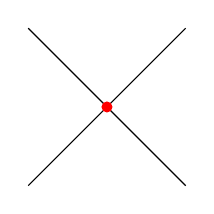
\begin{tikzpicture}[every node/.style={black, right}]
				\draw[name path=line 1] (-1, -1) -- (1,1);
				\draw[name path=line 2] (-1, 1) -- (1, -1);
				\fill[red,name intersections={of=line 1 and line 2,total=\t}]
					\foreach \s in {1,...,\t}{(intersection-\s) circle (2pt) node{}};
			\end{tikzpicture}
			\begin{tikzpicture}[every node/.style={black, right}]
				\draw[name path=line 1] (0, 1) -- (0,-1);
				\draw[name path=line 2] (-1, 0) -- (1, 0);
				\fill[red,name intersections={of=line 1 and line 2,total=\t}]
					\foreach \s in {1,...,\t}{(intersection-\s) circle (2pt) node{}};
			\end{tikzpicture}
			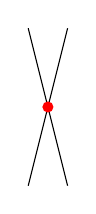
\begin{tikzpicture}[every node/.style={black, right}]
				\draw[name path=line 1] (-0.25, 1) -- (0.25,-1);
				\draw[name path=line 2] (0.25, 1) -- (-0.25, -1);
				\fill[red,name intersections={of=line 1 and line 2,total=\t}]
					\foreach \s in {1,...,\t}{(intersection-\s) circle (2pt) node{}};
			\end{tikzpicture}
		\end{figure}
	\newpage
	\section{Examples}
		\subsection*{1}

\end{document}
